%!TEX root = ../template.tex
%%%%%%%%%%%%%%%%%%%%%%%%%%%%%%%%%%%%%%%%%%%%%%%%%%%%%%%%%%%%%%%%%%%%
%% chapter4.tex
%% NOVA thesis document file
%%
%% Chapter with lots of dummy text
%%%%%%%%%%%%%%%%%%%%%%%%%%%%%%%%%%%%%%%%%%%%%%%%%%%%%%%%%%%%%%%%%%%%

\typeout{NT FILE chapter4.tex}%

\chapter{Implementation}
\label{cha:implementation}

In this chapter, we present the implementation of our system.
We begin by offering an overview of system's architecture,
before delving into the implementation of each module in depth.

\section{Architecture} % (fold)
\label{sec:architecture}


The system was built using a modular approach;
each module is entirely self-contained, making it simple to expand or replace system functionality.
The system architecture is split into two distinct areas: the runtime, and the pipeline.
The runtime architecture comprises all essential components to the system liveness,
whereas the pipeline architecture covers all components needed during the system's provisioning and development.

\subsection{Runtime Architecture} % (fold)
\label{sec:runtime_architecture}

The runtime environment is supported by Kubernetes,
a simplified configuration with three microservices is depicted in Figure ~\ref{fig:runtime},
in this example, we have one micro-service that has undergone three major API changes the accounts micro-service, and
two micro-services that rely on it, the inventory micro-service that was updated to account for the changes, and the shipping micro-service which is two versions behind.

In Kubernetes a microservice is internally accessible through the Service abstraction;
a Service defines a policy for accessing a logical set of Pods via a load balancer with a
unique IP address that can be discovered thorough an environment variable, or an DNS name.
The containers of a pod are selected in services policies by attributing names to their exposed ports and assigning the same name on the target port of the service policy.
In adapter containers we expose one port for each of the supported versions and name each port with the respective version.

We define one service for each major version that is still being consumed, as shown in Figure ~\ref{fig:runtime},
older versions are supported by the adapter, while the most up to date version is directly supported by the microservice app.
A consumer accesses a producer app via the service that haves the same version as the one that it's expected in the static code.
When a microservice app is upgraded via a rolling update \footnote{A rolling update gradually replaces old replicas with new replicas},
the services never become unavailable, they point either to the adapter containers or the application containers, depending on whether the affected pods finished the upgrade process,
whereas in the traditional approach all consumers would need to be upgraded in tandem with consumed services in order to avoid downtime.

The only novel module introduced in the runtime environment is the proxy adapter;
the forthcoming modules are either developer tools or are invoked on stages of the DevOps pipeline.

\begin{figure}[htbp]
    \centering
    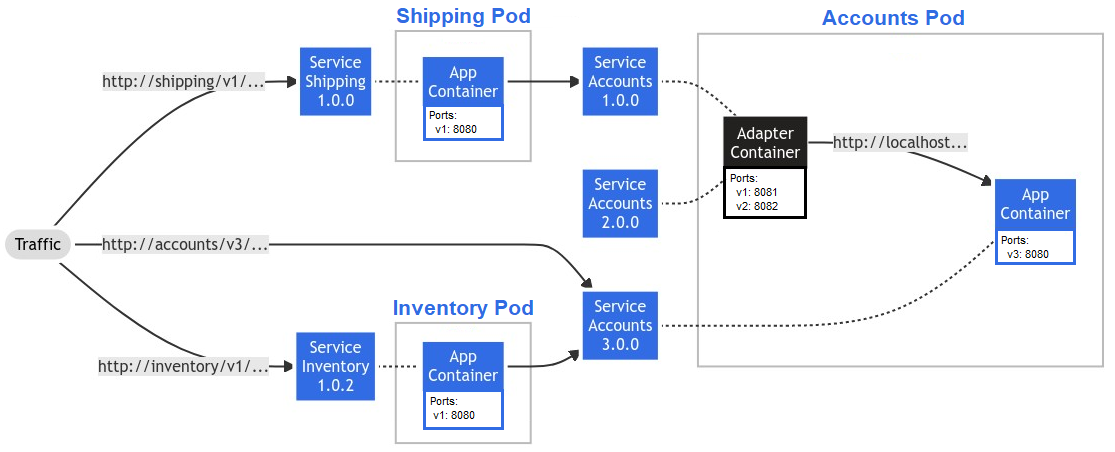
\includegraphics[height=2.4in]{runtime}
    \caption{Example of a runtime configuration}
    \label{fig:runtime}
\end{figure}

\subsection{DevOps Pipeline Architecture} % (fold)
\label{sec:devops_pipeline_architecture}

A proof-of-concept deployment pipeline as developed, its architecture is depicted in Figure ~\ref{fig:pipeline}.
The nodes on the left side of the graph represent the pipeline;
development stages are represented in green, while operational stages are represented in red.
The other nodes on the graph's reflect the resources used in each stage.
External resources are depicted in blue, while the novel modules developed in this thesis are depicted in black.
Two novel stages were introduced in the development phase: the writing of service contracts, and the specification of contract evolutions.
These two stages are skipped if a service only underwent changes that did not affect its API or dependencies.
We also introduced two novel stages in the development phase:
the verification of the service compatibility with the rest of the system, and the generation of adapter component.

The pipeline was developed using the Jenkins pipeline suite, each of the novel stages is supported by a distinct Java application that is pulled from version control
and executed directly on the pipeline, whereas the other stages are supported natively by the Jenkins suite toolkit.
The modules that enable each novel stage will be discussed in detail in the following section.

\begin{figure}[htbp]
    \centering
    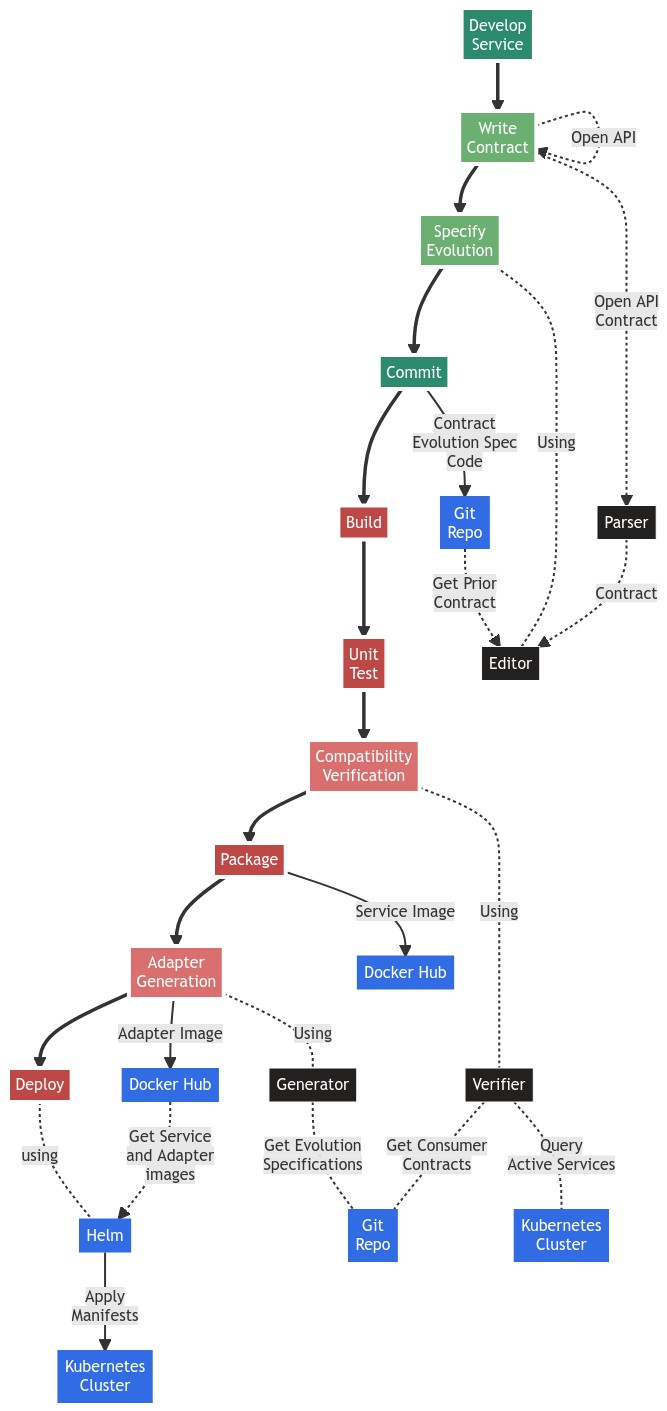
\includegraphics[height=9in]{DevOps}
    \caption{DevOps Pipeline}
    \label{fig:pipeline}
\end{figure}

\newpage

\section{Contract Representation} % (fold)
\label{sec:contract_representation}

The functionalities of web service's can be expressed with the
use Web Api Description Languages (WADL).
The OpenAPI specification is the most
widely adopted WADL for HTTP services, instead of designing yet another WADL, we
adopted the OpenAPI specification to support the needs of our implementation.
The OpenAPI initiative is on a continuous effort to develop API tooling on top of their specification, some of the supported tools of version 3.0 range from:

\begin{itemize}
    \item Auto Generators: Tools that parse code and turn it into an OpenAPI Specification document
    \item Mock Servers: Fake servers that take description document as input, then route incoming HTTP requests to example responses or dynamically generates examples.
    \item Data Validators: Verifies if API requests and responses are lining up with the API description.
    \item Security: Tools that can look out for attack vectors by inspecting OpenAPI descriptions.
    \item Converters: Various tools to convert to and from OpenAPI and other API description formats.
\end{itemize}

Designing a WADL tailored for this problem would be counterproductive because many teams already rely on the aforementioned tools,
and supporting an additional WADL would require the development of an extensive converter tool
that would need to be constantly maintained in order to support changes in new versions of the OpenApi and the new WADL specification's.

To represent records in messages, we chose the Json format, because of its simplicity and widespread adoption.
Json is a human-readable data-interchange format,
there are more performant formats that have binary representation,
however such formats are usually not supported by front-end frameworks and for the purpose of this prototype
we are not interested in measuring the performance of different object serialization protocols, since
there are already sources that provide comparisons in this regard between XML, Json, Protobuf, Thrift and other popular formats \cite{serializationBenchmark}.

The schema of JSON records must also be described,
the OpenAPI specification supports the description of records
in conjunction with the signature of HTTP endpoints.
Other Json schema specification languages, such as the Json-Schema project
exist, but using languages other than OpenApi would necessitate decoupling the specification of schemas from the specification
of http endpoints, which would require additional effort on the part of the developing team to maintain the cross-references
between each specification manifest, and their versions.

A snippet of a "Pet Store" OpenApi contract can be seen in Figure ~\ref{fig:open_contract}.
In this example we can view the specification of a JSON schema for a Pet data object,
as well the specification for an HTTP endpoint.
OpenApi allows properties to be defined robustly with specification of not only their type but also their format, as shown in line 31.

The types and formats of properties are standardized between object schemas and http parameters;
properties have the following data types: string, number, integer, boolean, array, and object;
while property formats are free-form, however there are established conventions for the most common formats.

The types and formats of properties are standardized between object schemas and http parameters;
properties have the following data types: string, number, integer, boolean, array, and object;
while property formats are free-form, there are established conventions for the most common types.

\begin{figure}[htbp]
    \centering
    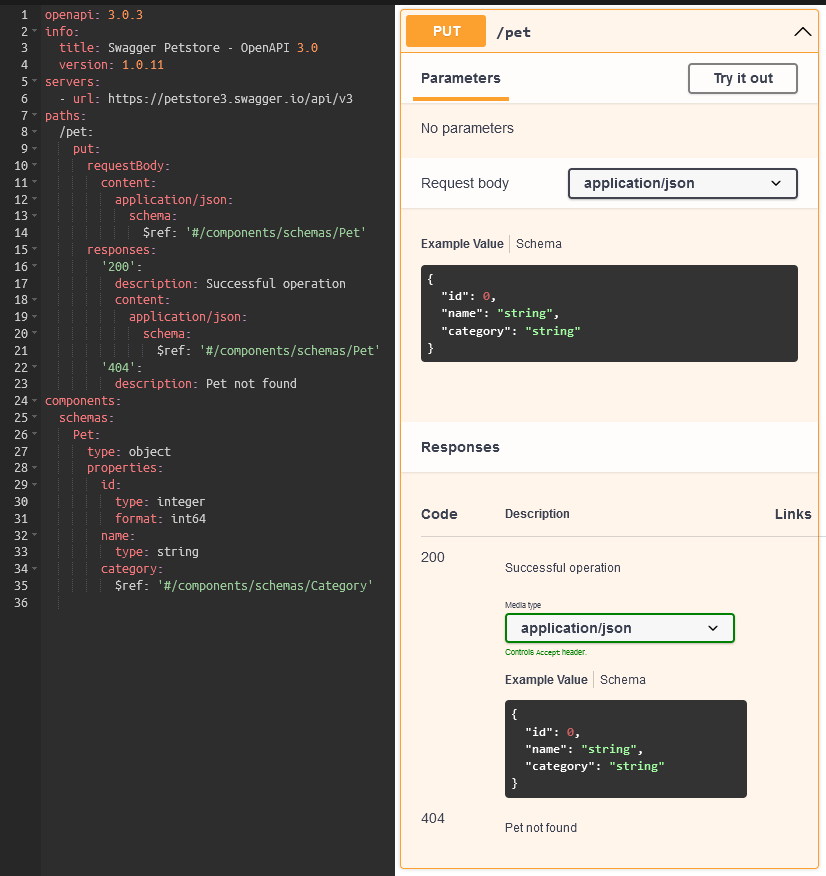
\includegraphics[height=6in]{openContract}
    \caption{OpenAPI Contract}
    \label{fig:open_contract}
\end{figure}

\newpage

The definition of the dependencies of a service is done using Helm.
Helm is package manager for Kubernetes that allows developers and operators to more easily package, configure, and deploy applications and services onto Kubernetes clusters.
A Chart is a Helm package, composed of a collection of files that describe a related set of Kubernetes resources.
The most significant components of a Chart are the:
\begin{itemize}
    \item The Chart.yaml that allows the definition of the Chart dependencies and other meta-information about the application such as its name and version.
    \item The Template's directory that contains incomplete Kubernetes manifests "Templates" such as Services, Deployments, DaemonSets, Namespaces and so on.
    \item The Values.yaml that contains key-value pairs used to complete the definition of each template, this values can be overridden later when the chart is deployed, the file is used to define the default values.
\end{itemize}
A single Chart might be used to deploy something simple, like a single kubernetes pod, or something complex, like a complete web app stack with HTTP servers, databases, caches, and so on.
The typical approach is to define an individual Chart for each distinct microservice, so that they can be upgraded individually.
If a single Chart is used to deploy multiple services it is no longer possible to represent accurately the dependencies of each service
in the chart definition, because the chart syntax doesn't allow the individual definition of the dependencies of each service, it only allows the declaration of the dependencies of the deployment as a whole.

An example of the definition of service dependencies can be seen in Figure ~\ref{fig:serviceDepedencies}.
The dependencies of a service are mapped indirectly, each dependency point to a Helm Chart that is implicitly associated with one service.
Helm Charts can be hosted on local or remote repositories.

\begin{figure}[htbp]
    \centering
    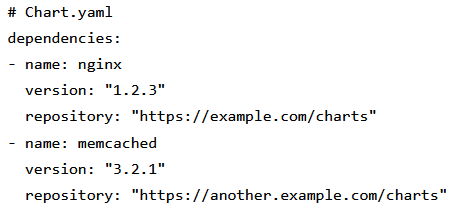
\includegraphics[height=2in]{serviceDepedencies}
    \caption{Helm Chart Dependencies Definition Example}
    \label{fig:serviceDepedencies}
\end{figure}

\newpage

The declaration of resources consumed by a service is defined in Chart template files,
for each deployment template we define the resources consumed by its containers by
defining the minimum amount of cpu and memory resources (represented on the requests key) and by setting a limit on these resources (represented on the limits key).
An example of the definition of a service resources can be seen in Figure ~\ref{fig:serviceResources}.

\begin{figure}[htbp]
    \centering
    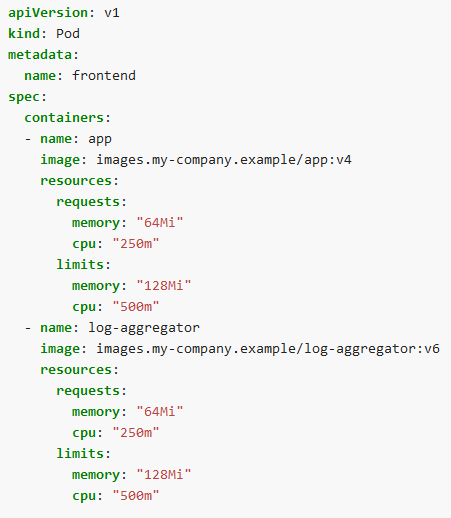
\includegraphics[height=3in]{serviceResources}
    \caption{Helm Template Resources Definition Example}
    \label{fig:serviceResources}
\end{figure}

\newpage

\section{Contract Interpretation} % (fold)
\label{sec:contract_interpretation}

The interpretation of contract specification is done in the Parser module.
This module is meant to be used as Java library by other modules,
it interprets contracts written in OpenApi format and provides a read-only Java interface
that is agnostic to the original specification format.
All the forthcoming modules operate under this interface not the OpenApi format.
Although we adopted the OpenApi format our solution is not dependent on it, this module provides a decoupling point.
This enables the specification of different contract to be written in different or even mixed WADL,
as long as the parser module is extended to support the new WADL's.

The actual parsing of OpenApi contracts is supported by the swagger-parser project, \textbf{[TODO: reference]}
which validates and parses OpenAPI definitions in JSON or YAML format into a Java POJO representation.

The interpretation of service resources and dependencies written in Helm charts is also supported by the Parser module under a separate interface.
The SnakeYAML library \textbf{[TODO: reference]} was used to parse the Charts.yaml and template files, into a Java class that implements a read-only Java interface.
The following are also decoupled from the Helm and Kubernetes API's they rely only on the read-only interfaces.

\newpage

\section{Evolution Representation} % (fold)
\label{sec:evolution_representation}

The evolution of contracts is represented in a custom description language.
The description only maps the details about the changed procedures of a service,
it is not necessary to map the evolutions in service dependencies and resource requirements because they can be inferred by comparing the last two contract versions.
The description language is hierarchical, and contains array elements.
The following Figure ~\ref{fig:evolution_yal} represents its structure, and gives an example.
Array elements are depicted by the [.] notation.

\begin{figure}[htbp]
    \centering
    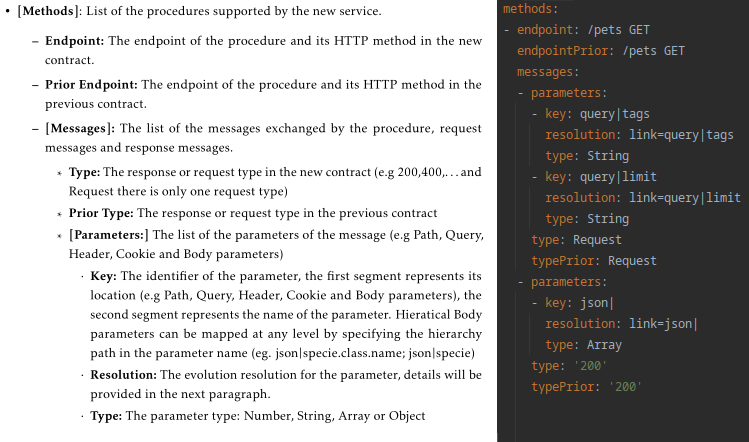
\includegraphics[height=3.75in]{evolutionYal}
    \caption{Evolution Specification Example}
    \label{fig:evolution_yal}
\end{figure}

As previously mentioned in the design chapter, resolutions can have one of three distinct types
DefaultValues, Link or Function.
The type of resolution is represented in the first segment of a resolution, while the second segment represents the resolution itself.

Link resolutions have the following format "link={Parameter Location}|{Parameter Name}", the parameter of the prior contract must be of the same type and format.

Default value resolutions have the following format "default=#Value", the value that must be of the same type and format.

Function resolutions are written as one line Java expressions that can use parameters of the previous contract, the
parameters are referenced by their location and name (eg. function= {{json|firstName}} + {{json|lastName}} ).
These references are replaced in the adapter implementation by their real value.

\newpage

\begin{figure}[htbp]
    \centering
    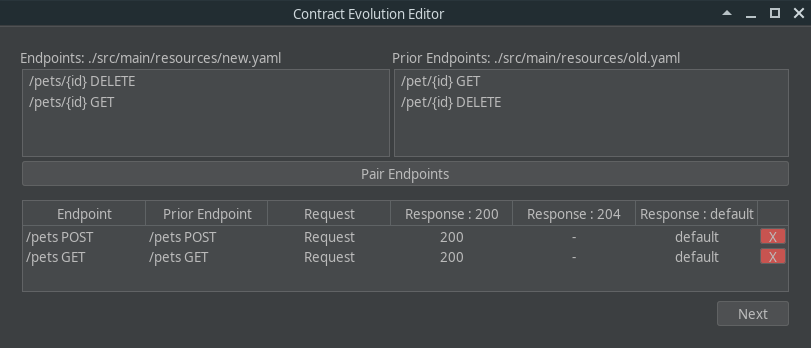
\includegraphics[height=2.4in]{editor2}
    \caption{Evolution Editor}
    \label{fig:editor2}
\end{figure}

\begin{figure}[htbp]
    \centering
    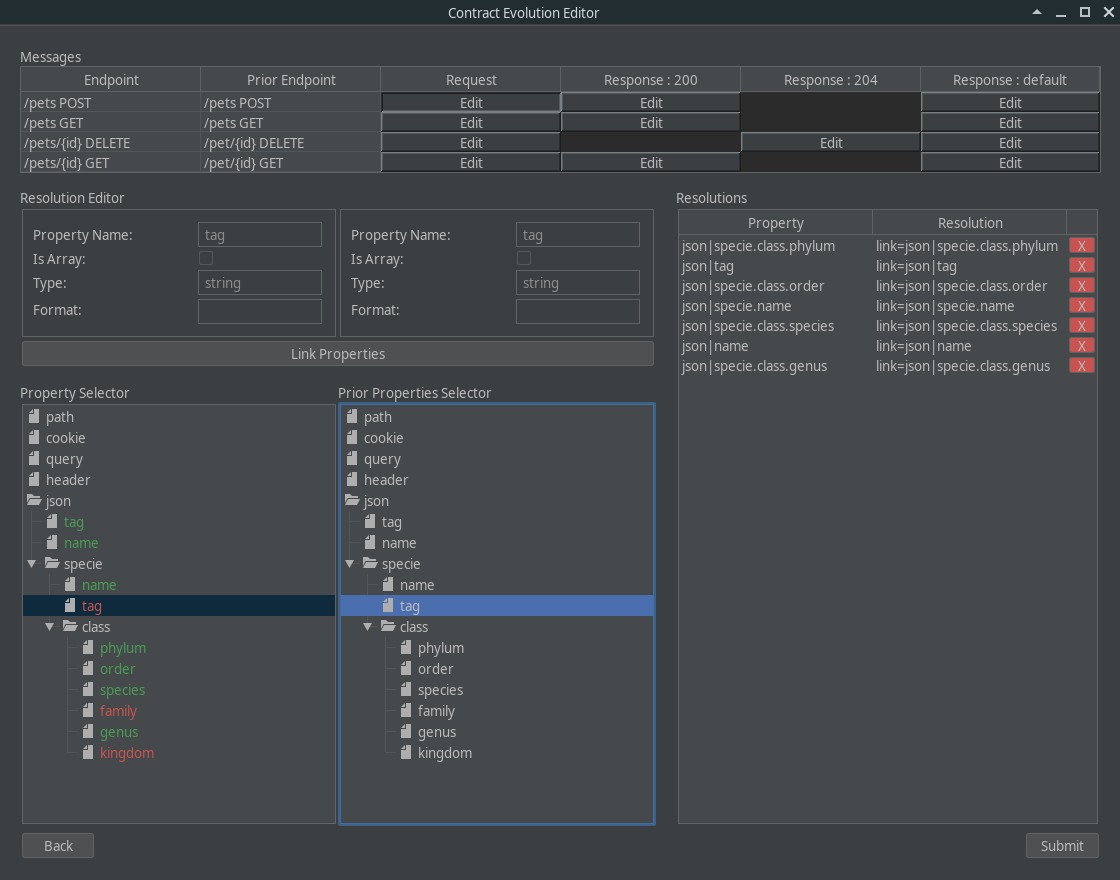
\includegraphics[height=4.4in]{editor1}
    \caption{Evolution Editor}
    \label{fig:editor1}
\end{figure}

To minimize the documentation effort we developed a GUI editor for the specification of evolutions.
The GUI editor was implemented as an IDE Plugin, the current implementation supports the Intellij IDE.
The editor compares two contract versions,
and automatically maps all the parameters that haven't changed from one version to the other, the
developer is left with the task of explicitly mapping the remaining procedures.
The editor starts by requesting the developer to map endpoints in the new contract to endpoints in the old contract,
afterwards the developer must edit each of the endpoint messages and specify a resolution for all the parameters that changed
in a contract, unresolved parameters are highlighted in red.
The right column holds the resolutions that were already mapped and uppermost left column allows the developer to write rules
for each unresolved parameter.
The developer can select leaf parameters in the hierarchy, or we can choose intermediate properties.
If he chooses an intermediate property and inputs resolution rule all child parameters are also resolved.
After all parameters are resolved the developer can submit the specification, and
the editor outputs an evolution spec with the same description language presented in the beginning of this section.


\newpage

\paragraph{Description}
\paragraph{Capabilities}
\paragraph{Limitations}
\paragraph{Dependencies}

\section{Verifier} % (fold)
\label{sec:verifier}

\paragraph{Description}
\paragraph{Capabilities}
\paragraph{Limitations}
\paragraph{Dependencies}

\section{Generator} % (fold)
\label{sec:generator}

\paragraph{Description}
\paragraph{Capabilities}
An HTTP contract contains the HTTP method, the
path, the parameter schema, and the location of parameters (path, query, header); the
proposed compatibility verification approaches supports all of these elements.

\paragraph{Limitations}
\paragraph{Dependencies}

\section{Adapter} % (fold)
\label{sec:adapter}

\paragraph{Tuning}. The demo application image was built using Ubuntu 18.04.6 as a base image and consists of Spring-boot microservice with a Apache Tomcat/9.0.65 http server.
In order to prevent the JVM from resizing and reallocating the heap memory while Tomcat is trying to serve requests and
calling garbage collector frequently, the JVM has started with a higher heap memory maximum, and the initial heap memory
size was set to the same value as its maximum memory size.
The maximum number of threads for Tomcat was set to 2000, in order to support a higher load of requests.

\paragraph{Description}
\paragraph{Capabilities}
\paragraph{Limitations}
\paragraph{Dependencies}

